\documentclass[11pt, oneside, numbers=nönddot]{scrbook}

\usepackage{style}

\def\Title{OSI 7 Schichtenmodell}	
\def\Subtitle{Layer 2}


\begin{document}


\titlehead{%
\begin{minipage}[c]{0.20\linewidth}

\includegraphics[width=0.8\linewidth]{htl_c_cmyk_rein.pdf}
\end{minipage}
\begin{minipage}[c]{0.5\linewidth}
\begin{center}
{\bfseries\sffamily\large Höhere  technische  Bundeslehranstalt\\
und  Bundesfachschule\\
{\normalsize im Hermann Fuchs Bundesschulzentrum} }
\end{center}
\end{minipage}
\begin{minipage}[c]{0.2\linewidth}
\hfill 
\includegraphics[width=0.8\linewidth]{htl-bildung-mit-zukunft.png}
\end{minipage}\\
}
\title{\vspace{4em}\Title}

\subtitle{\Subtitle}


\author{\\[2,5em] 
\emph{Erstellt von:} \\[0,5em]
Michel Rögl-Brunner, BEd
}
\date{\vspace{3\baselineskip}\small Letzte Änderung: \todayshort}

\begin{titlepage}	
\maketitle
\end{titlepage}
\IfFileExists{revisions.tex}{\clearpage\input{revisions.tex}}{}
\cleardoublepage
\pdfbookmark[1]{Inhaltsverzeichnis}{toc}
\tableofcontents
\clearpage
\pagenumbering{arabic}

\chapter{OSI-Modell und Layer 2}
\section{Grundlagen und Einordnung}
Layer 2 des OSI-Modells wird als \textit{Data Link Layer} oder \textbf{Sicherungsschicht} bezeichnet. Während Layer 1 ausschliesslich für die physikalische Übertragung von Bits zuständig ist, übernimmt Layer 2 die erste inhaltliche Strukturierung dieser Bits: Er fasst den rohen Bitstrom zu sinnvollen Einheiten zusammen, den sogenannten \textit{Frames} (Rahmen). Damit stellt er Layer 3 (dem Netzwerk-Layer) einen zuverlässigeren, adressierbaren Dienst zur Verfügung.

Die Protokolldateneinheit (PDU) auf Layer 2 ist der \textbf{Frame}. Im Gegensatz zu Layer 3, der mit logischen IP-Adressen arbeitet, verwendet Layer 2 \textbf{physikalische Adressen} -- die sogenannten MAC-Adressen. Diese sind eindeutig jedem Netzwerkinterface zugeordnet und ermöglichen die direkte Kommunikation innerhalb eines Netzsegments.

\subsubsection*{Aufgaben des Data Link Layer}
Layer 2 übernimmt mehrere klar definierte Aufgaben:
\begin{itemize}
\item \textbf{Framing:} Der Bitstrom von Layer 1 wird in strukturierte Frames unterteilt, die Anfang und Ende klar kennzeichnen.
\item \textbf{Physikalische Adressierung:} Jeder Frame enthält eine Quell- und eine Ziel-MAC-Adresse, sodass im Netzsegment festgestellt werden kann, woher ein Frame stammt und für wen er bestimmt ist.
\item \textbf{Fehlererkennung:} Durch Prüfsummen (z.\,B. CRC/FCS) kann Layer 2 erkennen, ob ein Frame während der Übertragung beschädigt wurde. Fehlerhafte Frames werden verworfen.
\item \textbf{Flusskontrolle:} In manchen Implementierungen regelt Layer 2 den Datenfluss zwischen Sender und Empfänger, um Überlastung zu vermeiden.
\item \textbf{Medienzugriffssteuerung (MAC):} Layer 2 regelt, wer wann auf das gemeinsame Übertragungsmedium zugreift. Dies ist besonders bei Halbduplex-Übertragungen wichtig.
\end{itemize}

\subsubsection*{Einordnung im OSI-Modell}
Layer 2 gliedert sich klassisch in zwei Unterschichten:
\begin{itemize}
\item \textbf{LLC (Logical Link Control):} Die obere Teilschicht sorgt für die verbindungsorientierte oder verbindungslose Kommunikation und stellt den Übergang zu Layer 3 her.
\item \textbf{MAC (Media Access Control):} Die untere Teilschicht verwaltet die physikalischen Adressen und steuert den Zugriff auf das Übertragungsmedium.
\end{itemize}

Im Alltag ist vor allem die MAC-Unterschicht präsent, da sie direkt mit den Ethernet-Frames und den MAC-Adressen verknüpft ist, mit denen wir täglich arbeiten.

\newpage

\section{MAC-Adressen}
\subsection{Aufbau und Struktur}
Eine MAC-Adresse (\textit{Media Access Control Address}) ist eine 48\,Bit (6\,Byte) lange physikalische Adresse, die jedem Netzwerkinterface weltweit eindeutig zugeordnet ist. Sie wird üblicherweise hexadezimal geschrieben, wobei die sechs Bytes durch Bindestriche oder Doppelpunkte getrennt werden:

\begin{center}
\texttt{AA:BB:CC:DD:EE:FF} \quad oder \quad \texttt{AA-BB-CC-DD-EE-FF}
\end{center}

Die 48 Bits teilen sich in zwei gleichgrosse Hälften:
\begin{itemize}
\item \textbf{OUI (Organizationally Unique Identifier):} Die ersten 3 Bytes (24\,Bit) kennzeichnen den Hersteller des Netzwerkinterfaces. Die IEEE vergibt diese Kennung an Hersteller. Beispiele: \texttt{00:1A:2B} steht für Cisco, \texttt{AC:DE:48} für ein Apple-Gerät.
\item \textbf{NIC-spezifischer Teil:} Die letzten 3 Bytes (24\,Bit) werden vom Hersteller frei vergeben und eindeutig jedem Interface zugeordnet.
\end{itemize}

\begin{figure}[H]
\centering
\IfFileExists{Work/Aufgaben/NWT/OSI-Modell/Layer2/images/mac_address_structure.png}{%
  
\includegraphics[width=0.75\textwidth]{Work/Aufgaben/NWT/OSI-Modell/Layer2/images/mac_address_structure.png}%
}{%
  \IfFileExists{images/mac_address_structure.png}{%
    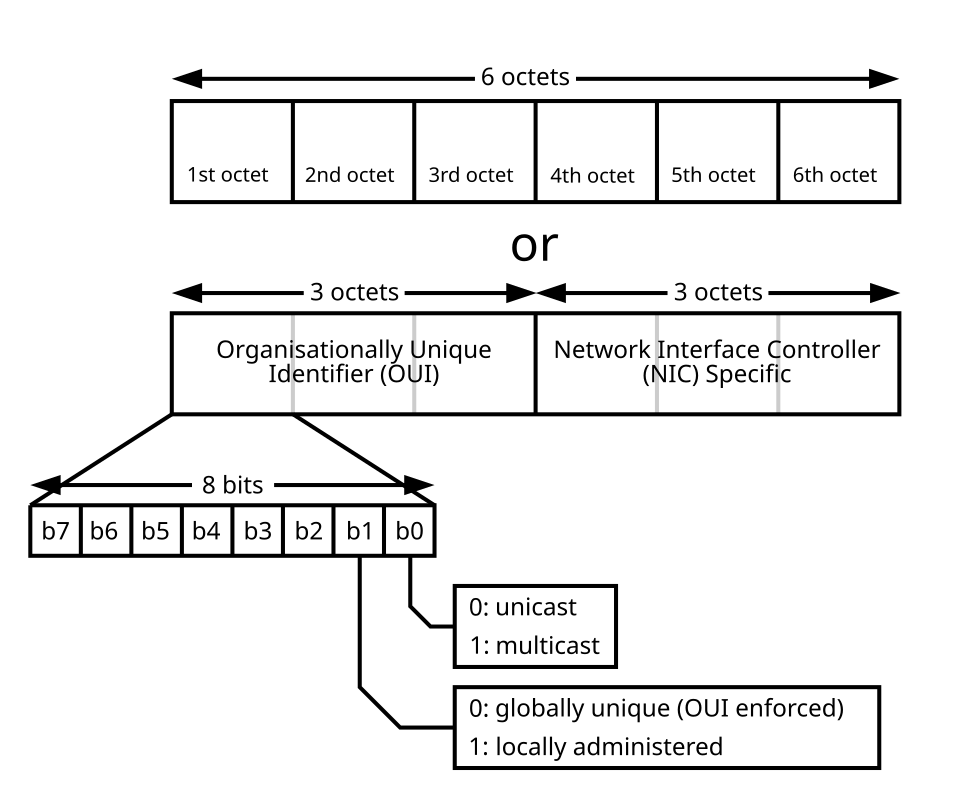
\includegraphics[width=0.75\textwidth]{images/mac_address_structure.png}%
  }{%
    \fbox{\parbox{0.85\textwidth}{Bild fehlt: \texttt{images/mac\_address\_structure.png}}}%
  }%
}
\caption{Aufbau einer MAC-48-Adresse mit OUI und Interface-Teil (Quelle: Wikimedia Commons, Datei: MAC-48\_Address.svg, CC BY-SA 2.5)}
\end{figure}

\subsection{Sonderbits in der MAC-Adresse}
Das erste Byte der MAC-Adresse enthält zwei besondere Steuerbits, die im niedrigstwertigen Bereich liegen:

\begin{itemize}
\item \textbf{Bit 0 (Unicast/Multicast-Bit):} Ist dieses Bit \texttt{0}, handelt es sich um eine \textit{Unicast}-Adresse -- der Frame ist für genau ein Gerät bestimmt. Ist es \texttt{1}, ist es eine \textit{Multicast}-Adresse: Der Frame richtet sich an eine Gruppe von Geräten, die sich für diese Multicast-Gruppe registriert haben.
\item \textbf{Bit 1 (G/L-Bit, Global/Locally Administered):} Ist dieses Bit \texttt{0}, ist die Adresse global eindeutig (vom Hersteller vergeben). Ist es \texttt{1}, wurde die Adresse lokal manuell konfiguriert oder per Software zugewiesen.
\end{itemize}

\subsection{Adresstypen im Überblick}

\begin{longtable}{|p{3.5cm}|p{4.5cm}|p{5.5cm}|}
\hline
\textbf{Adresstyp} & \textbf{Beispiel} & \textbf{Bedeutung} \\
\hline
Unicast & \texttt{AC:DE:48:12:34:56} & Genau ein Empfänger-Interface \\
\hline
Multicast & \texttt{01:00:5E:xx:xx:xx} & Gruppe von Empfängern (IPv4-Multicast) \\
\hline
Broadcast & \texttt{FF:FF:FF:FF:FF:FF} & Alle Geräte im Netzsegment \\
\hline
Locally Administered & z.\,B. \texttt{02:xx:xx:xx:xx:xx} & Manuell vergeben, lokal gültig \\
\hline
\end{longtable}

\subsection{Broadcast-Adresse}
Die Adresse \texttt{FF:FF:FF:FF:FF:FF} ist die Layer-2-Broadcast-Adresse. Ein Frame mit dieser Zieladresse wird von \textbf{allen Geräten} im selben Netzsegment angenommen und verarbeitet. Typische Anwendungsfälle sind ARP-Anfragen (\textit{Address Resolution Protocol}), bei denen ein Gerät nach der MAC-Adresse zu einer bekannten IP-Adresse fragt, ohne den Empfänger vorher zu kennen.

Broadcasts werden von Switches weitergeleitet (innerhalb des VLANs), aber von Routern nicht -- ein Router bildet eine \textit{Broadcast-Domain-Grenze}. Das Konzept der Broadcast-Domain ist daher eng mit Layer 2 verknüpft.

\subsection{MAC-Adressen in der Praxis}
Obwohl MAC-Adressen theoretisch weltweit eindeutig und fest in der Hardware gespeichert sind, lassen sich viele Betriebssysteme und Netzwerkadapter so konfigurieren, dass sie eine andere (``gespoofde'') MAC-Adresse nach aussen signalisieren. Dies kann für Tests oder Datenschutzmassnahmen nützlich sein, birgt aber auch Sicherheitsrisiken (z.\,B. Umgehung von MAC-basierten Zugangsbeschränkungen). Deshalb sollte eine rein MAC-basierte Sicherheitskontrolle immer durch weitere Mechanismen ergänzt werden.

\newpage

\section{Ethernet}
\subsection{Geschichte und Standard}
Ethernet ist die heute bei weitem am häufigsten eingesetzte LAN-Technologie und bildet die technische Grundlage für den Grossteil moderner Netzwerkkommunikation. Die Ursprünge liegen in den 1970er Jahren bei Xerox PARC, wo Robert Metcalfe und seine Kollegen das Grundprinzip des CSMA/CD-basierten Medienzugriffs entwickelten. \textbf{1980} präsentierten Xerox, Intel und DEC gemeinsam den ersten Ethernet-Standard (``DIX Ethernet'' oder ``Ethernet II'') mit einer Datenrate von 10\,Mbit/s.

\textbf{1983} veröffentlichte das IEEE den Standard \textit{IEEE 802.3}, der Ethernet formal standardisierte. Seitdem wurde der Standard stetig weiterentwickelt: von 10\,Mbit/s über 100\,Mbit/s (Fast Ethernet, 802.3u), 1\,Gbit/s (Gigabit Ethernet, 802.3z/ab), 10\,Gbit/s (802.3ae) bis hin zu 100\,Gbit/s und mehr für Rechenzentren. Heute ist Ethernet nicht mehr auf Koaxialkabel beschränkt, sondern läuft auf Twisted-Pair-Kabeln, Glasfaser und in Datenzentren auf speziellen Hochgeschwindigkeitsverbindungen.

\subsection{Der Ethernet-Frame}
Die Grundstruktur des Ethernet-II-Frames (der im Alltag verwendeten Variante) sieht folgendermassen aus:

\begin{figure}[H]
\centering
\IfFileExists{Work/Aufgaben/NWT/OSI-Modell/Layer2/images/ethernet_frame.png}{%
  
\includegraphics[width=0.95\textwidth]{Work/Aufgaben/NWT/OSI-Modell/Layer2/images/ethernet_frame.png}%
}{%
  \IfFileExists{images/ethernet_frame.png}{%
    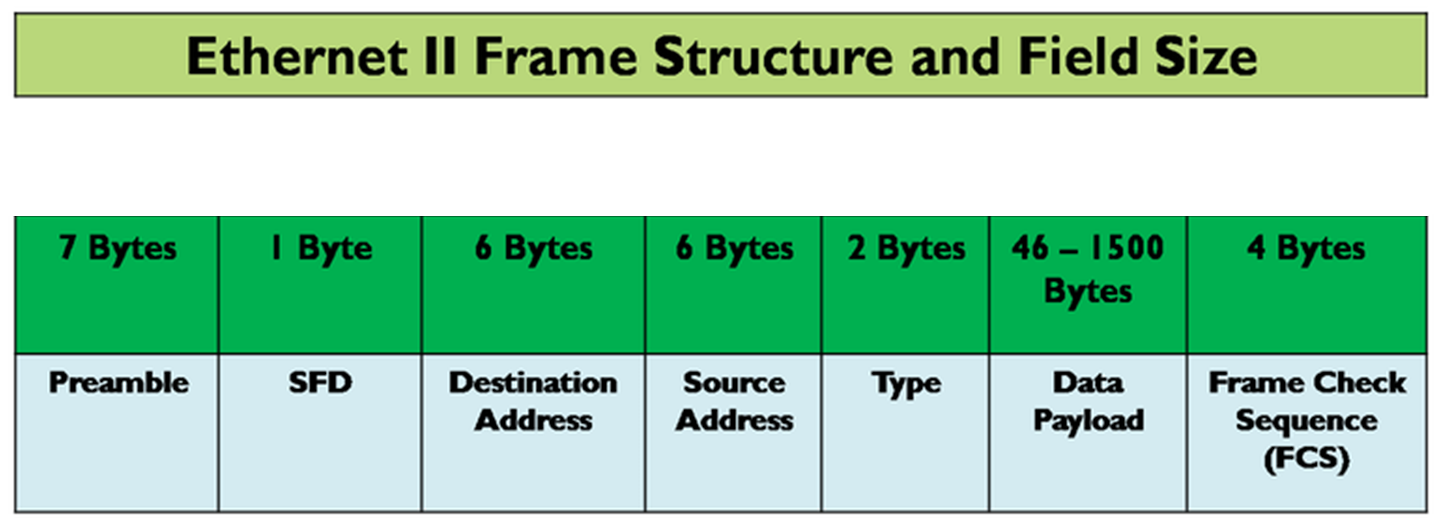
\includegraphics[width=0.95\textwidth]{images/ethernet_frame.png}%
  }{%
    \fbox{\parbox{0.85\textwidth}{Bild fehlt: \texttt{images/ethernet\_frame.png}}}%
  }%
}
\caption{Ethernet-II-Frame-Struktur (Quelle: Wikimedia Commons, Datei: Ethernet\_II\_Frame\_Structure.png, CC BY-SA 4.0)}
\end{figure}

\begin{longtable}{|p{3.2cm}|p{2.2cm}|p{7.8cm}|}
\hline
\textbf{Feld} & \textbf{Grösse} & \textbf{Bedeutung} \\
\hline
Preamble & 7 Byte & Abwechselnde 1/0-Bits zur Taktsynchronisation des Empfängers \\
\hline
SFD (Start Frame Delimiter) & 1 Byte & Markiert den Beginn des eigentlichen Frames (\texttt{10101011}) \\
\hline
Destination MAC & 6 Byte & MAC-Adresse des Empfängers (Unicast, Multicast oder Broadcast) \\
\hline
Source MAC & 6 Byte & MAC-Adresse des Senders \\
\hline
EtherType / Länge & 2 Byte & Wert $\geq$ 1536: EtherType (Protokoll-ID); Wert $<$ 1536: Nutzdatenlänge (802.3) \\
\hline
Payload (Nutzdaten) & 46--1500 Byte & Nutzdaten, z.\,B. ein IP-Paket. Mindestens 46 Byte (ggf. mit Padding aufgefüllt) \\
\hline
FCS (Frame Check Sequence) & 4 Byte & CRC-32-Prüfsumme über Dst/Src/EtherType/Payload zur Fehlererkennung \\
\hline
\end{longtable}

Preamble und SFD werden in der Regel nicht als Teil des eigentlichen Frames gezählt -- die Mindestgrösse des ``eigentlichen'' Frames beträgt deshalb \textbf{64 Byte} (6+6+2+46+4), die maximale Grösse \textbf{1518 Byte} (ohne 802.1Q-Tag). Frames unter 64 Byte gelten als \textit{Runt Frames} und werden verworfen.

\subsection{EtherType -- Protokollkennung}
Das EtherType-Feld im Ethernet-Frame teilt dem Empfänger mit, welches Layer-3-Protokoll im Payload steckt. Wichtige Werte:

\begin{longtable}{|l|l|}
\hline
\textbf{EtherType-Wert} & \textbf{Protokoll} \\
\hline
\texttt{0x0800} & IPv4 \\
\hline
\texttt{0x86DD} & IPv6 \\
\hline
\texttt{0x0806} & ARP (Address Resolution Protocol) \\
\hline
\texttt{0x8100} & 802.1Q VLAN-Tag \\
\hline
\texttt{0x8847} & MPLS (Unicast) \\
\hline
\end{longtable}

\subsection{Jumbo Frames}
In Standardnetzwerken ist die maximale Nutzlast (MTU) auf 1500 Byte begrenzt. In Hochleistungs-Umgebungen (z.\,B. Rechenzentren, Storage-Netzwerke) werden häufig \textit{Jumbo Frames} mit einer MTU von bis zu 9000 Byte eingesetzt. Das reduziert den Overhead durch weniger Frame-Header pro übertragener Datenmenge und entlastet die CPU. Wichtig: Alle beteiligten Geräte im Pfad müssen Jumbo Frames unterstützen und entsprechend konfiguriert sein.

\subsection{Half-Duplex, Full-Duplex und CSMA/CD}
In frühen Ethernet-Netzwerken arbeiteten alle Geräte an einem gemeinsamen Koaxialkabel oder über einen Hub im \textbf{Halbduplex-Modus}: Senden und Empfangen war nicht gleichzeitig möglich. Um Kollisionen zu handhaben, wurde \textit{CSMA/CD} (\textit{Carrier Sense Multiple Access with Collision Detection}) eingesetzt:

\begin{enumerate}
\item Gerät horcht, ob das Medium frei ist (\textit{Carrier Sense}).
\item Ist es frei, beginnt es zu senden (\textit{Multiple Access}).
\item Kollision erkannt: Alle Sender stoppen, senden ein Jam-Signal und warten eine zufällige Zeit (\textit{Backoff}), bevor sie es erneut versuchen (\textit{Collision Detection}).
\end{enumerate}

Moderne geswitchte Netzwerke arbeiten fast ausschliesslich im \textbf{Full-Duplex-Modus}: Senden und Empfangen erfolgen gleichzeitig über separate Leitungspaare. Kollisionen sind damit praktisch ausgeschlossen, und CSMA/CD spielt in diesem Kontext keine Rolle mehr. Die maximale theoretische Datenrate wird vollständig ausgenutzt.

\newpage

\section{Switches}
\subsection{Was ist ein Switch?}
Ein \textbf{Switch} ist ein aktives Layer-2-Netzwerkgerät, das Frames anhand von MAC-Adressen gezielt an den richtigen Port weiterleitet. Im Gegensatz zu einem \textbf{Hub}, der jeden empfangenen Frame einfach an alle anderen Ports dupliziert (``flooding''), trifft ein Switch eine intelligente Weiterleitungsentscheidung: Er lernt, welche MAC-Adresse an welchem Port erreichbar ist, und sendet Frames nur an den jeweils benötigten Port.

\begin{figure}[H]
\centering
\IfFileExists{Work/Aufgaben/NWT/OSI-Modell/Layer2/images/switch_vs_hub.png}{%
  
\includegraphics[width=0.95\textwidth]{Work/Aufgaben/NWT/OSI-Modell/Layer2/images/switch_vs_hub.png}%
}{%
  \IfFileExists{images/switch_vs_hub.png}{%
    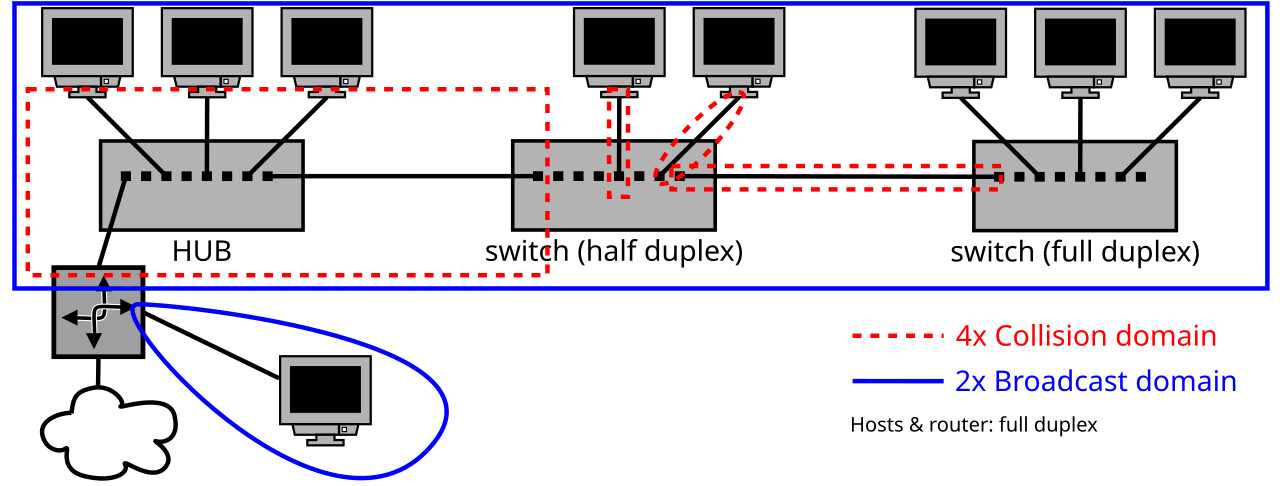
\includegraphics[width=0.95\textwidth]{images/switch_vs_hub.png}%
  }{%
    \fbox{\parbox{0.85\textwidth}{Bild fehlt: \texttt{images/switch\_vs\_hub.png}}}%
  }%
}
\caption{Kollisions- und Broadcast-Domains bei Hub, Switch (Halbduplex) und Switch (Vollduplex) (Quelle: Wikimedia Commons, Datei: Ethernet-broadcast-collision.svg, CC BY-SA 4.0)}
\end{figure}

\subsection{Die drei Grundoperationen eines Switches}
Jeder Layer-2-Switch arbeitet nach denselben drei Grundprinzipien:

\subsubsection{Learning (Lernen)}
Wenn ein Frame am Switch eintrifft, liest der Switch die \textbf{Quell-MAC-Adresse} des Frames aus und trägt sie zusammen mit dem eingehenden Port und einem Zeitstempel in die \textit{MAC-Adresstabelle} (auch \textit{CAM-Tabelle}) ein. So weiss der Switch in Zukunft, an welchem Port dieses Gerät erreichbar ist.

\subsubsection{Flooding (Fluten)}
Ist die \textbf{Ziel-MAC-Adresse} eines eingehenden Frames noch \textbf{nicht} in der MAC-Adresstabelle vorhanden (unbekanntes Ziel), sendet der Switch den Frame an \textbf{alle Ports ausser dem Eingangsport}. Ebenso werden Broadcast-Frames (\texttt{FF:FF:FF:FF:FF:FF}) und Multicast-Frames (sofern kein IGMP Snooping konfiguriert ist) stets geflutet. Dieses Verfahren garantiert, dass der Frame sein Ziel auch dann erreicht, wenn der Switch den entsprechenden Port noch nicht kennt.

\subsubsection{Forwarding / Filtering (Weiterleiten und Filtern)}
Ist die Ziel-MAC-Adresse in der Tabelle bekannt, leitet der Switch den Frame \textbf{gezielt} an den zugehörigen Port weiter. Liegt Quell- und Ziel-Port auf demselben Port (z.\,B. beide Geräte hängen an einem weiteren Switch), wird der Frame verworfen (\textit{Filtering}), da der Empfänger den Frame bereits direkt erhalten hat.

\subsection{Collision Domains und Broadcast Domains}
Ein wichtiger Vorteil von Switches gegenüber Hubs liegt im Umgang mit Kollisions- und Broadcast-Domains:

\begin{longtable}{|p{4cm}|p{5.2cm}|p{4.2cm}|}
\hline
\textbf{Gerät} & \textbf{Collision Domain} & \textbf{Broadcast Domain} \\
\hline
Hub & Eine gemeinsame Collision Domain für alle Ports & Eine gemeinsame Broadcast Domain \\
\hline
Switch & Jeder Port bildet eine eigene Collision Domain & Alle Ports in einem VLAN teilen eine Broadcast Domain \\
\hline
Router & Jeder Port bildet eine eigene Collision Domain & Jeder Port bildet eine eigene Broadcast Domain \\
\hline
\end{longtable}

Durch die Segmentierung der Collision Domains eliminiert ein Switch Kollisionen bei Full-Duplex-Betrieb vollständig. Die Broadcast Domain bleibt jedoch zunächst erhalten -- alle Ports in einem VLAN empfangen Broadcasts. Erst ein Router oder eine Layer-3-Switch-Funktion grenzt Broadcast-Domains voneinander ab.

\newpage

\section{Switching Table (MAC-Adresstabelle)}
\subsection{Aufbau der Tabelle}
Die MAC-Adresstabelle (auch \textit{CAM-Table}, \textit{Forwarding Database} oder kurz FDB) ist das Kernelement eines Switches. Sie enthält die Zuordnung von MAC-Adressen zu Ports. Ein typischer Eintrag besteht aus folgenden Feldern:

\begin{longtable}{|p{3.5cm}|p{9.5cm}|}
\hline
\textbf{Feld} & \textbf{Bedeutung} \\
\hline
MAC-Adresse & Die gelernte Quell-MAC-Adresse des Endgeräts \\
\hline
Port & Der physikalische Port, an dem das Gerät mit dieser MAC-Adresse zuletzt einen Frame gesendet hat \\
\hline
VLAN & Das VLAN, in dem dieser Eintrag gültig ist (MAC-Adressen können in verschiedenen VLANs getrennt verwaltet werden) \\
\hline
Alter (Age) & Zeitstempel oder Zähler seit dem letzten Auftreten; nach Ablauf des \textit{Aging-Timers} wird der Eintrag gelöscht \\
\hline
\end{longtable}

Auf einem Cisco-Switch lässt sich die MAC-Adresstabelle beispielsweise mit folgendem Befehl anzeigen:
\begin{verbatim}
Switch# show mac address-table
\end{verbatim}

\subsection{Ablauf: Wie lernt ein Switch?}
Das folgende Beispiel zeigt Schritt für Schritt, wie ein Switch mit vier angeschlossenen Geräten (PC-A an Port 1, PC-B an Port 2, PC-C an Port 3, PC-D an Port 4) seine MAC-Tabelle aufbaut:

\begin{enumerate}
\item \textbf{Ausgangszustand:} Die MAC-Tabelle ist leer. Kein Gerät ist bisher bekannt.
\item \textbf{PC-A sendet einen Frame an PC-C.} Der Switch empfängt den Frame an Port\,1 und trägt die Quell-MAC von PC-A in die Tabelle ein: \texttt{MAC-A $\rightarrow$ Port 1}. Die Ziel-MAC von PC-C ist unbekannt $\Rightarrow$ Flooding an Ports 2, 3 und 4.
\item \textbf{PC-C antwortet.} Der Switch empfängt den Antwort-Frame an Port\,3 und lernt: \texttt{MAC-C $\rightarrow$ Port 3}. Die Ziel-MAC ist jetzt bekannt (Port\,1) $\Rightarrow$ Forwarding nur an Port\,1.
\item \textbf{PC-B sendet an PC-A.} Der Switch lernt \texttt{MAC-B $\rightarrow$ Port 2}, leitet den Frame direkt an Port\,1 weiter.
\item \textbf{Ergebnis:} Der Switch kennt nun MAC-A, MAC-B und MAC-C. Zukünftige Frames zwischen diesen Geräten werden gezielt weitergeleitet, ohne andere Ports zu belasten. PC-D ist noch unbekannt.
\end{enumerate}

\subsection{Aging-Timer}
Einträge in der MAC-Tabelle sind nicht dauerhaft. Nach einer definierten Zeit ohne Aktivität -- dem \textit{Aging-Timer} (typisch 300 Sekunden) -- werden Einträge automatisch gelöscht. Hintergrund: Geräte können den Port wechseln (z.\,B. Laptop umgesteckt), und der Switch müsste sonst immer noch den alten, falschen Port verwenden. Durch das Aging bleibt die Tabelle dynamisch und aktuell.

\subsection{CAM-Table-Overflow (MAC-Flooding-Angriff)}
Die MAC-Adresstabelle eines Switches hat eine begrenzte Grösse (abhängig vom Modell: oft einige tausend bis hunderttausend Einträge). Ein Angreifer kann durch gezieltes Senden von Frames mit vielen unterschiedlichen (gefälschten) Quell-MAC-Adressen die Tabelle vollständig füllen (\textit{MAC-Flooding}). Ist die Tabelle voll, kann der Switch neue Adressen nicht mehr lernen und muss alle Frames fluten -- er verhält sich wie ein Hub. Dadurch kann der Angreifer den Datenverkehr aller anderen Geräte mitlesen.

Schutz bieten \textit{Port Security}-Funktionen auf verwalteten Switches, die die maximale Anzahl von MAC-Adressen pro Port begrenzen und bei Überschreitung den Port abschalten oder Alarm auslösen.

\newpage

\section{VLANs -- Virtual Local Area Networks}
\subsection{Was ist ein VLAN?}
Ein \textbf{VLAN} (\textit{Virtual Local Area Network}) erlaubt es, ein physikalisches Netzwerk logisch in mehrere voneinander isolierte Netzsegmente aufzuteilen, ohne dass dafür separate physikalische Hardware erforderlich ist. Geräte in verschiedenen VLANs können \textbf{nicht direkt auf Layer 2 kommunizieren} -- sie verhalten sich so, als wären sie an physikalisch getrennten Switches angeschlossen. Für die Kommunikation zwischen VLANs ist ein Layer-3-Gerät (Router oder Layer-3-Switch) erforderlich.

Typische Gründe für den Einsatz von VLANs:
\begin{itemize}
\item \textbf{Sicherheit:} Trennung von Abteilungen (z.\,B. Verwaltung, Produktion, Gäste-WLAN).
\item \textbf{Performance:} Reduzierung der Broadcast-Domain -- weniger Geräte empfangen Broadcasts, die sie nicht benötigen.
\item \textbf{Flexibilität:} Logische Gruppenbildung unabhängig von der physikalischen Position der Geräte.
\item \textbf{Netzmanagement:} Einfacheres Troubleshooting durch übersichtliche Segmentierung.
\end{itemize}

\subsection{IEEE 802.1Q -- VLAN-Tagging}
Der Standard \textit{IEEE 802.1Q} definiert, wie VLAN-Informationen in Ethernet-Frames kodiert werden. Dazu wird ein 4\,Byte grosser \textbf{VLAN-Tag} in den Frame eingefügt, direkt nach der Quell-MAC-Adresse:

\begin{figure}[H]
\centering
\IfFileExists{Work/Aufgaben/NWT/OSI-Modell/Layer2/images/vlan_8021q.png}{%
  
\includegraphics[width=0.95\textwidth]{Work/Aufgaben/NWT/OSI-Modell/Layer2/images/vlan_8021q.png}%
}{%
  \IfFileExists{images/vlan_8021q.png}{%
    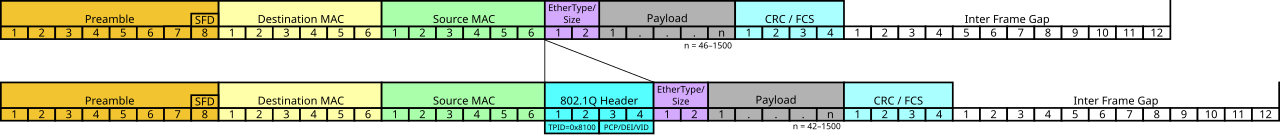
\includegraphics[width=0.95\textwidth]{images/vlan_8021q.png}%
  }{%
    \fbox{\parbox{0.85\textwidth}{Bild fehlt: \texttt{images/vlan\_8021q.png}}}%
  }%
}
\caption{Ethernet-Frame vor und nach Einfügen des 802.1Q-VLAN-Tags (Quelle: Wikimedia Commons, Datei: Ethernet\_802.1Q\_Insert.svg, CC BY-SA 3.0)}
\end{figure}

Der 4-Byte-Tag gliedert sich in folgende Felder:

\begin{longtable}{|p{2.8cm}|p{1.8cm}|p{8.7cm}|}
\hline
\textbf{Feld} & \textbf{Grösse} & \textbf{Bedeutung} \\
\hline
TPID & 16\,Bit & Tag Protocol Identifier: immer \texttt{0x8100}, kennzeichnet den Frame als 802.1Q-getaggt \\
\hline
PCP & 3\,Bit & Priority Code Point (IEEE 802.1p): Priorisierung des Frames (0--7, 7 = höchste Priorität) \\
\hline
DEI & 1\,Bit & Drop Eligible Indicator: Kennzeichnet Frames, die bei Überlast bevorzugt verworfen werden dürfen \\
\hline
VID & 12\,Bit & VLAN Identifier: Nummer des VLANs (0--4095, nutzbar: 1--4094) \\
\hline
\end{longtable}

Da der Tag den Frame vergrössert, steigt die maximale Framegrösse bei 802.1Q-getaggten Frames auf \textbf{1522 Byte}.

\subsection{Access Port und Trunk Port}
Auf einem Switch unterscheidet man grundsätzlich zwei Port-Typen:

\begin{itemize}
\item \textbf{Access Port:} Verbindet ein Endgerät (PC, Drucker, IP-Telefon) mit dem Switch. Der Port gehört genau einem VLAN an. Eingehende Frames werden vom Switch intern mit dem VLAN-Tag versehen; ausgehende Frames werden ohne Tag an das Endgerät weitergegeben. Das Endgerät selbst ``sieht'' keinen 802.1Q-Tag.
\item \textbf{Trunk Port:} Verbindet zwei Switches (oder einen Switch mit einem Router/Layer-3-Switch) miteinander. Über einen Trunk können Frames \textbf{mehrerer VLANs gleichzeitig} übertragen werden. Jeder Frame trägt dabei seinen 802.1Q-Tag, damit das empfangende Gerät weiss, zu welchem VLAN der Frame gehört.
\end{itemize}

Diese Unterscheidung ist fundamental: Würde man einen Trunk-Port fälschlicherweise als Access-Port konfigurieren (oder umgekehrt), entstünden VLAN-Leckagen oder Konnektivitätsprobleme. Korrekte Portkonfiguration ist daher ein zentraler Bestandteil des Switch-Managements.

\newpage

\section{Spanning Tree Protocol (STP)}
\subsection{Das Problem: Loops im Layer-2-Netz}
In professionellen Netzwerken werden Switches häufig redundant verkabelt: Gibt es zwei physikalische Pfade zwischen zwei Switches, ist einer davon als Backup gedacht. Auf Layer 3 lösen Routing-Protokolle solche Redundanzen elegant -- auf \textbf{Layer 2 hingegen entstehen ohne Schutzmaßnahme gefährliche Schleifen (Loops)}.

Ein Layer-2-Loop hat fatale Folgen:
\begin{itemize}
\item \textbf{Broadcast-Sturm:} Broadcast-Frames werden endlos im Kreis gesendet und amplifiziert, bis das Netz zusammenbricht.
\item \textbf{MAC-Tabellen-Instabilität:} Switches ``sehen'' dieselbe MAC-Adresse abwechselnd an verschiedenen Ports (je nachdem, von welcher Seite der Loop gerade kommt) und aktualisieren die Tabelle ständig (\textit{MAC-Flapping}).
\item \textbf{Netzausfall:} Die Bandbreite wird vollständig durch Schleifenverkehr verbraucht; reguläre Frames können nicht mehr übertragen werden.
\end{itemize}

\subsection{STP-Grundprinzip}
Das \textbf{Spanning Tree Protocol (STP)}, standardisiert in \textit{IEEE 802.1D}, löst dieses Problem, indem es alle redundanten Pfade automatisch erkennt und genau einen davon blockiert, bis der aktive Pfad ausfällt. Der Algorithmus berechnet einen loop-freien Baum (\textit{Spanning Tree}), der alle Switches miteinander verbindet.

Die wichtigsten Konzepte:
\begin{itemize}
\item \textbf{Root Bridge:} Jedes STP-Netz hat genau eine Root Bridge -- der ``Wurzel-Switch'' des Baums. Die Root Bridge wird durch die niedrigste \textit{Bridge ID} bestimmt (Kombination aus Priorität und MAC-Adresse). Alle anderen Switches orientieren sich an ihr.
\item \textbf{Root Port:} Jeder Nicht-Root-Switch wählt den Port mit dem günstigsten Pfad zur Root Bridge als \textit{Root Port} -- dieser ist stets im Forwarding-Zustand.
\item \textbf{Designated Port:} Pro Netzsegment gibt es genau einen \textit{Designated Port}, der Frames in Richtung Root Bridge weiterleitet. Auch dieser ist im Forwarding-Zustand.
\item \textbf{Blocked Port:} Alle übrigen Ports, die zu Loops führen würden, werden in den \textit{Blocking}-Zustand versetzt. Sie empfangen zwar STP-Nachrichten (BPDUs), leiten aber keine regulären Datenpakete weiter.
\end{itemize}

\begin{figure}[H]
\centering
\IfFileExists{Work/Aufgaben/NWT/OSI-Modell/Layer2/images/stp_topology.png}{%
  
\includegraphics[width=0.65\textwidth]{Work/Aufgaben/NWT/OSI-Modell/Layer2/images/stp_topology.png}%
}{%
  \IfFileExists{images/stp_topology.png}{%
    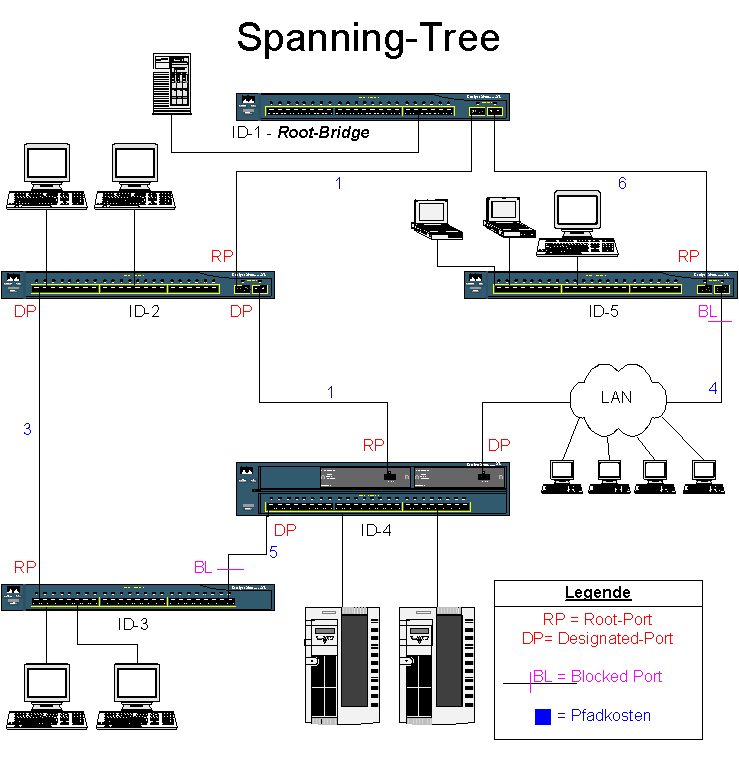
\includegraphics[width=0.65\textwidth]{images/stp_topology.png}%
  }{%
    \fbox{\parbox{0.85\textwidth}{Bild fehlt: \texttt{images/stp\_topology.png}}}%
  }%
}
\caption{Beispiel einer Spanning-Tree-Topologie in einem geswitchten Ethernet (Quelle: Wikimedia Commons, Datei: Spanning\_tree\_topology.png, CC BY-SA 3.0)}
\end{figure}

\begin{figure}[H]
\centering
\IfFileExists{Work/Aufgaben/NWT/OSI-Modell/Layer2/images/stp_at_work.png}{%
  
\includegraphics[width=0.5\textwidth]{Work/Aufgaben/NWT/OSI-Modell/Layer2/images/stp_at_work.png}%
}{%
  \IfFileExists{images/stp_at_work.png}{%
    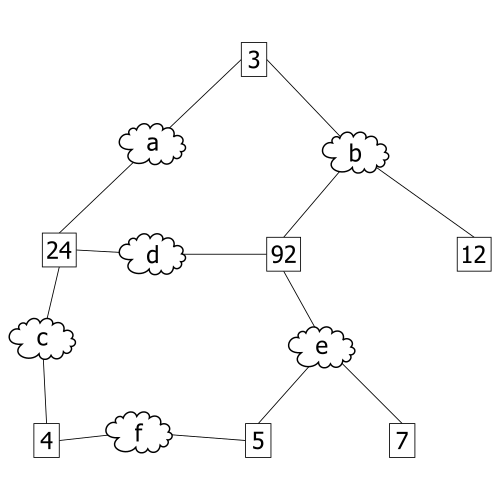
\includegraphics[width=0.5\textwidth]{images/stp_at_work.png}%
  }{%
    \fbox{\parbox{0.85\textwidth}{Bild fehlt: \texttt{images/stp\_at\_work.png}}}%
  }%
}
\caption{STP in Aktion: Root Bridge und blockierter Port (Quelle: Wikimedia Commons, Datei: Spanning\_tree\_protocol\_at\_work\_1.svg, CC BY 3.0)}
\end{figure}

\subsection{STP-Port-Zustände}
Ein STP-Port durchläuft beim Aktivieren mehrere Zustände:

\begin{longtable}{|p{3cm}|p{10cm}|}
\hline
\textbf{Zustand} & \textbf{Beschreibung} \\
\hline
Blocking & Port empfängt BPDUs, leitet keine Frames weiter. Schutz vor Loops. \\
\hline
Listening & Port verarbeitet BPDUs aktiv, lernt aber noch keine MAC-Adressen. \\
\hline
Learning & Port lernt MAC-Adressen, leitet aber noch keine Frames weiter. \\
\hline
Forwarding & Port leitet Frames normal weiter. Regulärer Betriebszustand. \\
\hline
Disabled & Port ist administrativ deaktiviert. \\
\hline
\end{longtable}

Der Übergang von Blocking bis Forwarding dauert bei klassischem STP (802.1D) insgesamt bis zu \textbf{50 Sekunden}. In modernen Netzwerken ist das zu langsam.

\subsection{RSTP -- Rapid Spanning Tree Protocol}
\textit{IEEE 802.1w} (Rapid STP, RSTP) ist die Weiterentwicklung von STP und bietet deutlich schnellere Konvergenz -- typischerweise unter \textbf{1--2 Sekunden}. RSTP verwendet denselben Algorithmus, optimiert aber die Aushandlung zwischen Switches durch einen direkten Handshake-Mechanismus statt dem reinen Timeout-basierten Ansatz. RSTP ist vollständig rückwärtskompatibel zu STP.

In aktuellen Netzwerken und auf modernen Switches wird RSTP standardmässig verwendet. \textit{MSTP} (Multiple Spanning Tree Protocol, 802.1s) geht noch einen Schritt weiter und erlaubt es, verschiedene VLANs auf unterschiedliche Spanning Trees zu mappen, um Lastverteilung über redundante Links zu ermöglichen.

\newpage

\section{Zusammenfassung}
Layer 2 des OSI-Modells bildet die erste intelligente Schicht der Netzwerkkommunikation. Während Layer 1 rohe Bits überträgt, strukturiert, adressiert und kontrolliert Layer 2 diese Daten auf Segment-Ebene. Die zentralen Konzepte dieses Layers sind eng miteinander verknüpft:

\textbf{MAC-Adressen} bilden die Grundlage für alle Layer-2-Kommunikation. Ihre 48-Bit-Struktur mit OUI und Interface-Teil, kombiniert mit den Sonderfunktionen für Unicast, Multicast und Broadcast, ermöglicht eine eindeutige Adressierung innerhalb eines Netzsegments.

\textbf{Ethernet} und der zugehörige Frame-Aufbau standardisieren die Struktur jeder übertragenen Dateneinheit. Die Felder Destination-MAC, Source-MAC, EtherType und FCS machen den Frame selbstbeschreibend und prüfbar. Mit über 40 Jahren Weiterentwicklung ist Ethernet heute die dominierende LAN-Technologie von 10\,Mbit/s bis 400\,Gbit/s.

\textbf{Switches} ersetzen Hubs als zentrales Layer-2-Verbindungsgerät. Durch gezieltes Forwarding auf Basis der MAC-Adresstabelle werden Kollisionsdomänen eliminiert und das Netz effizienter genutzt. Die drei Grundoperationen Learning, Flooding und Forwarding sind die Kernmechanismen jedes Switches.

\textbf{VLANs} erlauben die logische Segmentierung eines physikalischen Netzes. Das 802.1Q-Tagging ermöglicht den Transport mehrerer VLANs über einen einzigen Trunk-Link. Access Ports und Trunk Ports definieren, wie Endgeräte und Switch-zu-Switch-Verbindungen konfiguriert werden.

\textbf{STP und RSTP} schützen Layer-2-Netze vor Loops und den damit verbundenen Broadcast-Stürmen. STP blockiert redundante Pfade automatisch und aktiviert sie im Fehlerfall -- RSTP macht das deutlich schneller und ist heute der Standard in professionellen Netzwerken.

\begin{longtable}{|p{3.2cm}|p{10cm}|}
\hline
\textbf{Konzept} & \textbf{Kernaussage} \\
\hline
PDU & Frame (Layer 2), enthält Src-MAC, Dst-MAC, Nutzdaten, FCS \\
\hline
MAC-Adresse & 48\,Bit, 6\,Byte, OUI + Interface-Teil, global eindeutig \\
\hline
Ethernet & IEEE 802.3, Frame-Struktur, EtherType, Full-Duplex, bis 400\,Gbit/s \\
\hline
Switch & Layer-2-Gerät, lernt MAC-Adressen, leitet Frames gezielt weiter \\
\hline
Switching Table & MAC $\rightarrow$ Port-Zuordnung, Aging-Timer, CAM-Table \\
\hline
VLAN & Logische Netztrennung, 802.1Q-Tag, Access/Trunk-Port \\
\hline
STP / RSTP & Loop-Vermeidung, Root Bridge, Blocked Port, Konvergenz \\
\hline
\end{longtable}

Für das Verständnis aller höheren Protokollschichten ist Layer 2 unverzichtbar. IP-Pakete auf Layer 3, TCP-Segmente auf Layer 4 -- sie alle reisen innerhalb von Ethernet-Frames über das Netzwerk. Wer Layer 2 versteht, versteht, wie Daten tatsächlich von Port zu Port fliessen.


\end{document}
